% !TeX program = pdflatex
\documentclass[12pt,a4paper]{article}

\usepackage[utf8]{inputenc}
\usepackage[T1]{fontenc}
\usepackage[polish]{babel}
\usepackage{graphicx}
\usepackage{amsmath, amssymb}
\usepackage{float}
\usepackage{geometry}
\usepackage{booktabs}
\usepackage{caption}
\usepackage{subcaption}
\usepackage{pgfplots}
\usepackage{hyperref}
\usepackage{icomma}

\geometry{margin=2.5cm}
\setlength{\parindent}{1.2cm}
\setlength{\parskip}{0.5em}
\linespread{1.2}
\pgfplotsset{compat=1.18}

\hypersetup{
	colorlinks=true,
	linkcolor=black,
	filecolor=black,
	urlcolor=blue,
	pdftitle={Sprawozdanie SA - Cw 1},
	pdfpagemode=FullScreen,
}

\begin{document}
	
	\begin{titlepage}
		\centering
		\Huge \textbf{Sprawozdanie z ćwiczeń laboratoryjnych}\\[0.5cm]
		\Large z przedmiotu: \textit{Sterowanie Analogowe}\\[2cm]
		
		\begin{tabular}{|p{6cm}|p{10cm}|}
			\hline
			\textbf{Numer ćwiczenia:} & 1 \\ \hline
			\textbf{Tytuł ćwiczenia:} & Identyfikacja obiektów dynamicznych \\ \hline
			\textbf{Imię, nazwisko i numer albumu:} &
			\begin{tabular}[t]{@{}l@{}}
				Mateusz Kuczerowski 197900\\
				Kewin Kisiel 197866\\
			\end{tabular} \\ \hline
			\textbf{Data pomiarów:} & 9.10.2025 \\ \hline
			\textbf{Data oddania:} & 15.10.2025 \\ \hline
			\textbf{Ocena:} & \\ \hline
		\end{tabular}\\[2cm]
		
		\vfill
		\textbf{Prowadzący:} dr inż. Piotr Fiertek\\[0.2cm]
		\textbf{Grupa laboratoryjna:} 1A\\[1cm]
	\end{titlepage}
	
	\section{Cel ćwiczenia}
	Celem ćwiczenia było zapoznanie się z czasowymi i częstotliwościowymi metodami identyfikacji obiektów dynamicznych oraz praktyczne wyznaczenie modeli matematycznych opisujących ich zachowanie. W ramach zajęć analizowano odpowiedzi różnych typów układów dynamicznych na wymuszenia skokowe i sygnały harmoniczne, co pozwoliło na określenie ich podstawowych parametrów, takich jak wzmocnienie, stała czasowa, opóźnienie transportowe, współczynnik tłumienia czy pulsacja naturalna.
	
	\section{Przebieg ćwiczenia}
	Podczas ćwiczenia przeprowadzono identyfikację kilku obiektów dynamicznych o znanych transmitancjach operatorowych: układu inercyjnego pierwszego rzędu, układu inercyjnego pierwszego rzędu z opóźnieniem transportowym, układu całkującego, układu drugiego rzędu oraz układu nieminimalnofazowego. Dla każdego z nich wykonano pomiary odpowiedzi czasowych oraz charakterystyk częstotliwościowych (amplitudowych i fazowych). W trakcie zajęć wykorzystano stanowisko pomiarowe zbudowane z zestawu analogowych modeli procesów przemysłowych (ZAMPP), generatora funkcji, częstościomierza oraz oscyloskopu dwukanałowego. Zarejestrowane dane zostały następnie przetworzone i poddane analizie w środowisku MATLAB, gdzie z użyciem odpowiednich skryptów dokonano numerycznej identyfikacji parametrów poszczególnych modeli.
	
	\newpage
	\section{Pomiary i analiza wyników}
	Poniżej przedstawiono zdjęcia z przeprowadzonych pomiarów w trakcie laboratorium.
	
	\begin{figure}[H]
		\centering
		\begin{subfigure}[b]{0.48\textwidth}
			\centering
			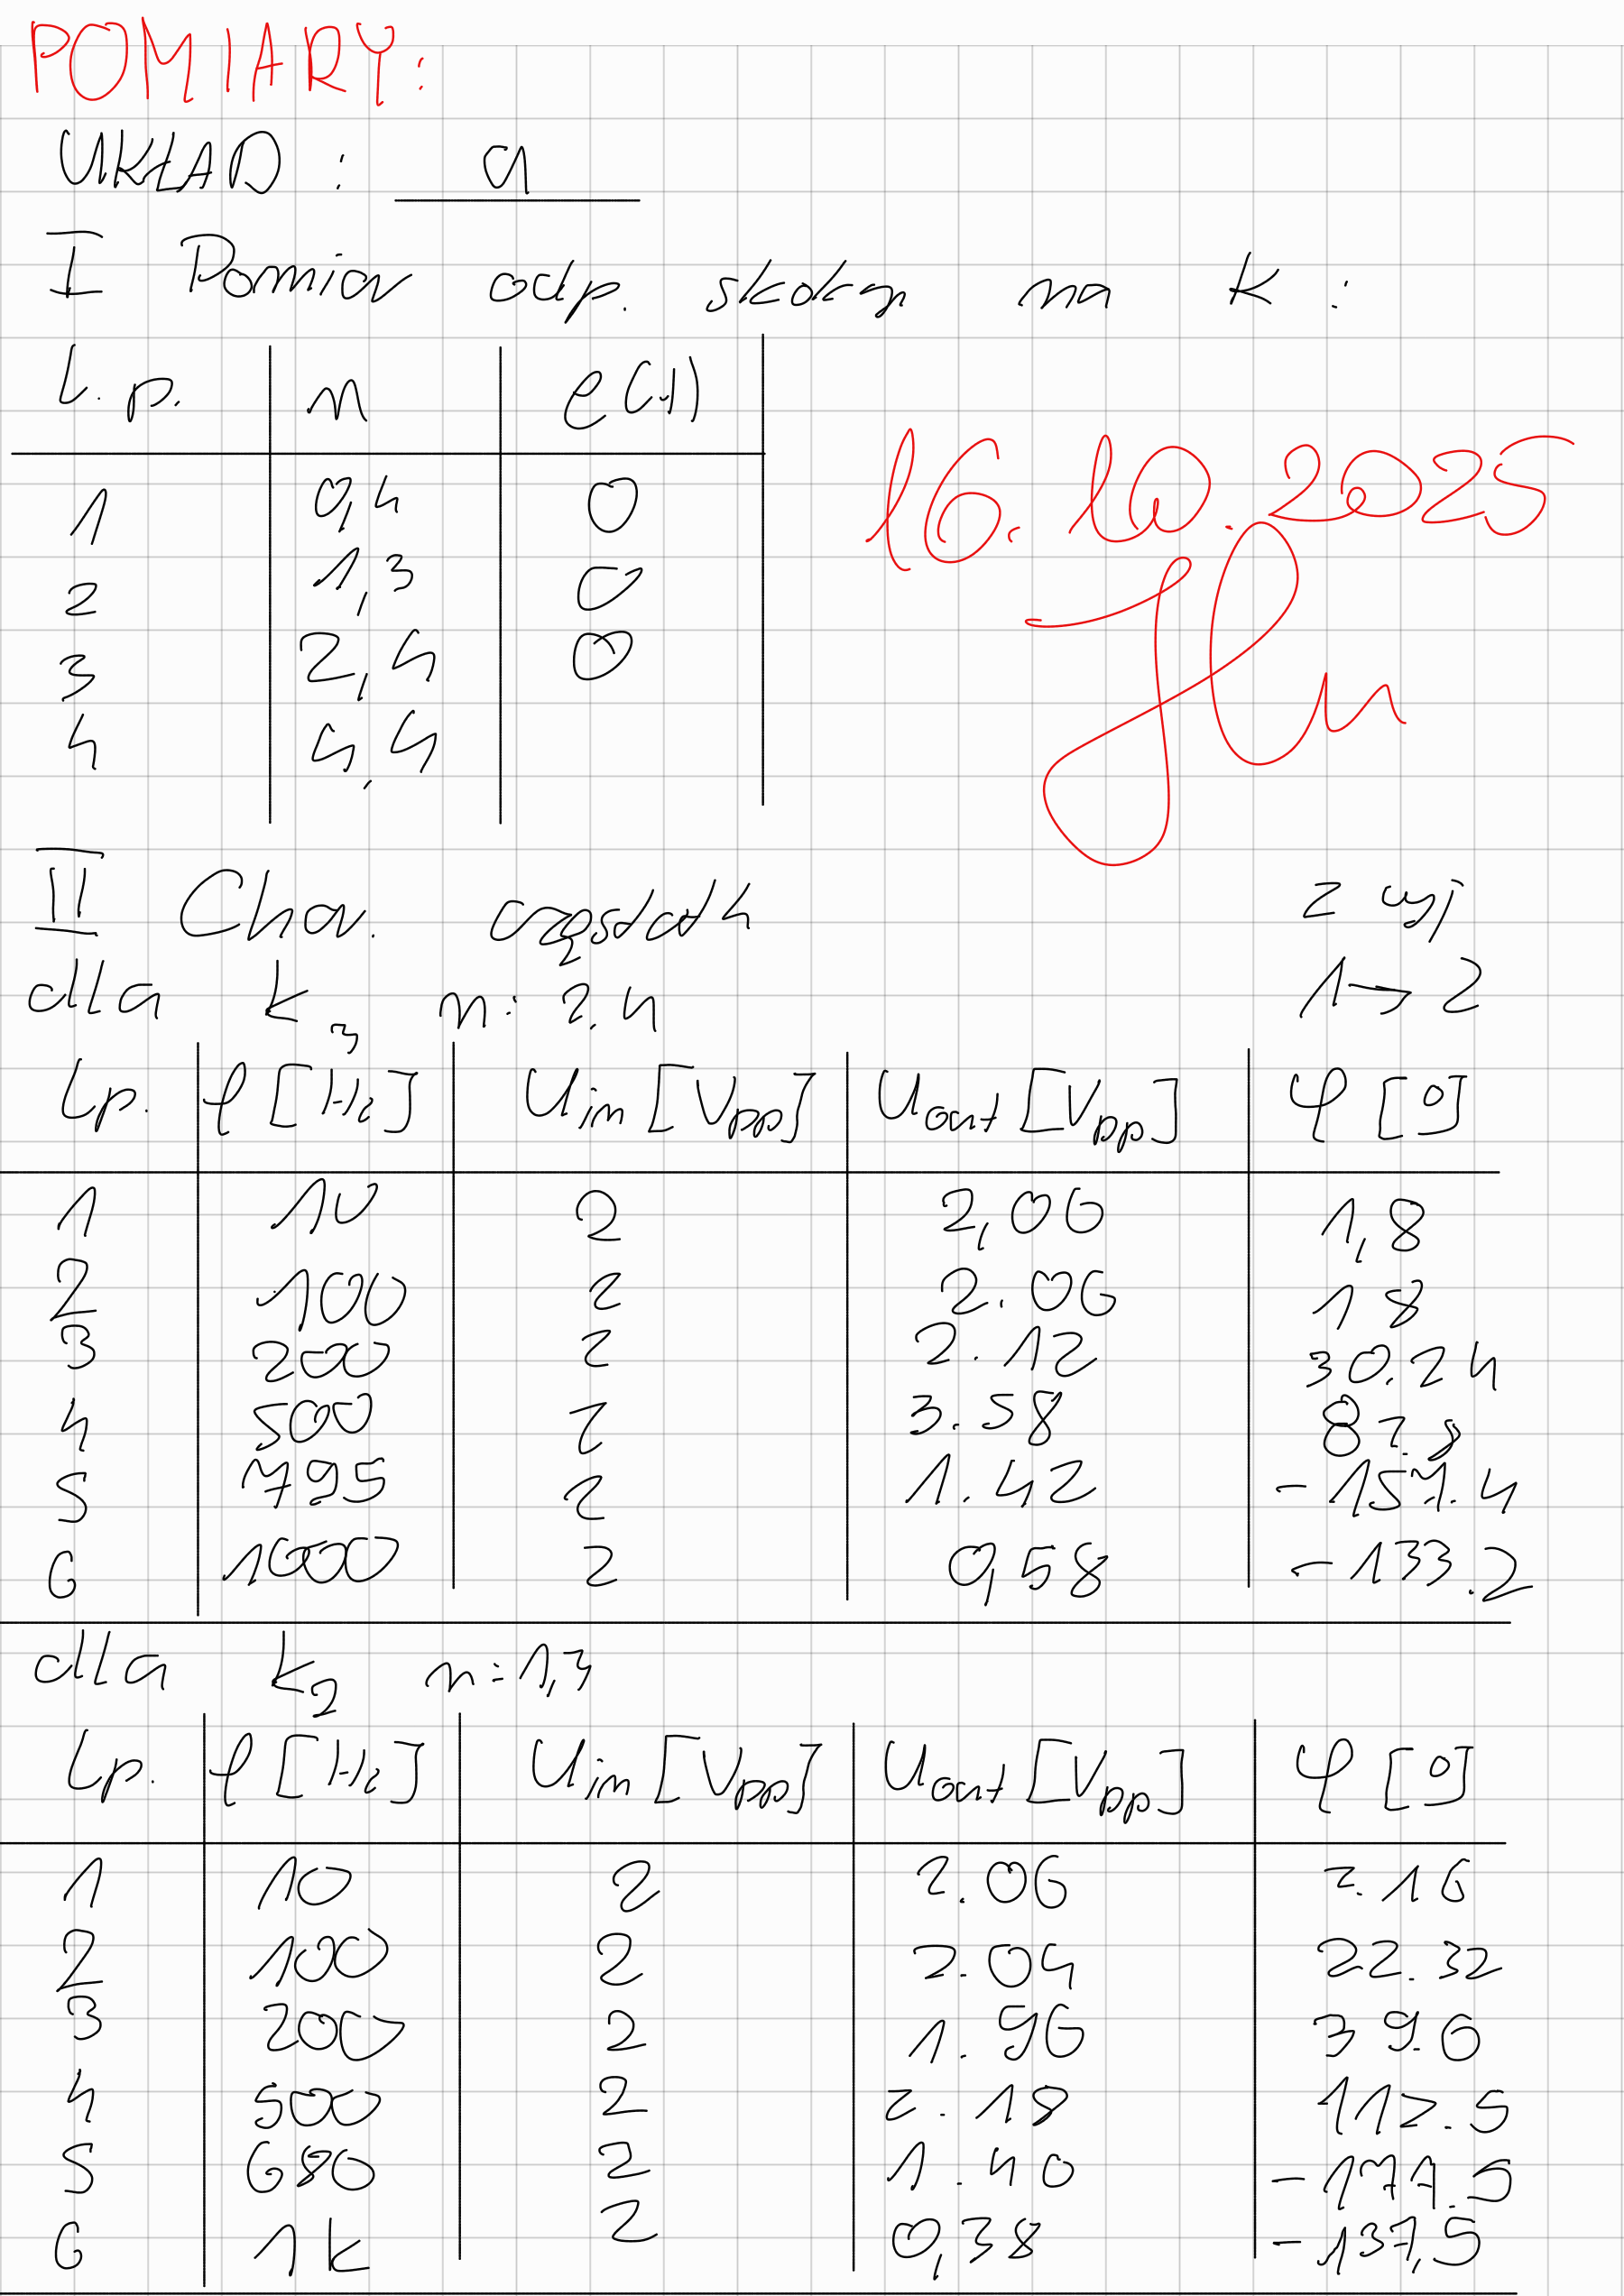
\includegraphics[width=\textwidth]{zdjecia/1.png}
			\caption{Zdjęcie pomiarów 1.}
			\label{fig:pomiar1}
		\end{subfigure}
		\hfill
		\begin{subfigure}[b]{0.48\textwidth}
			\centering
			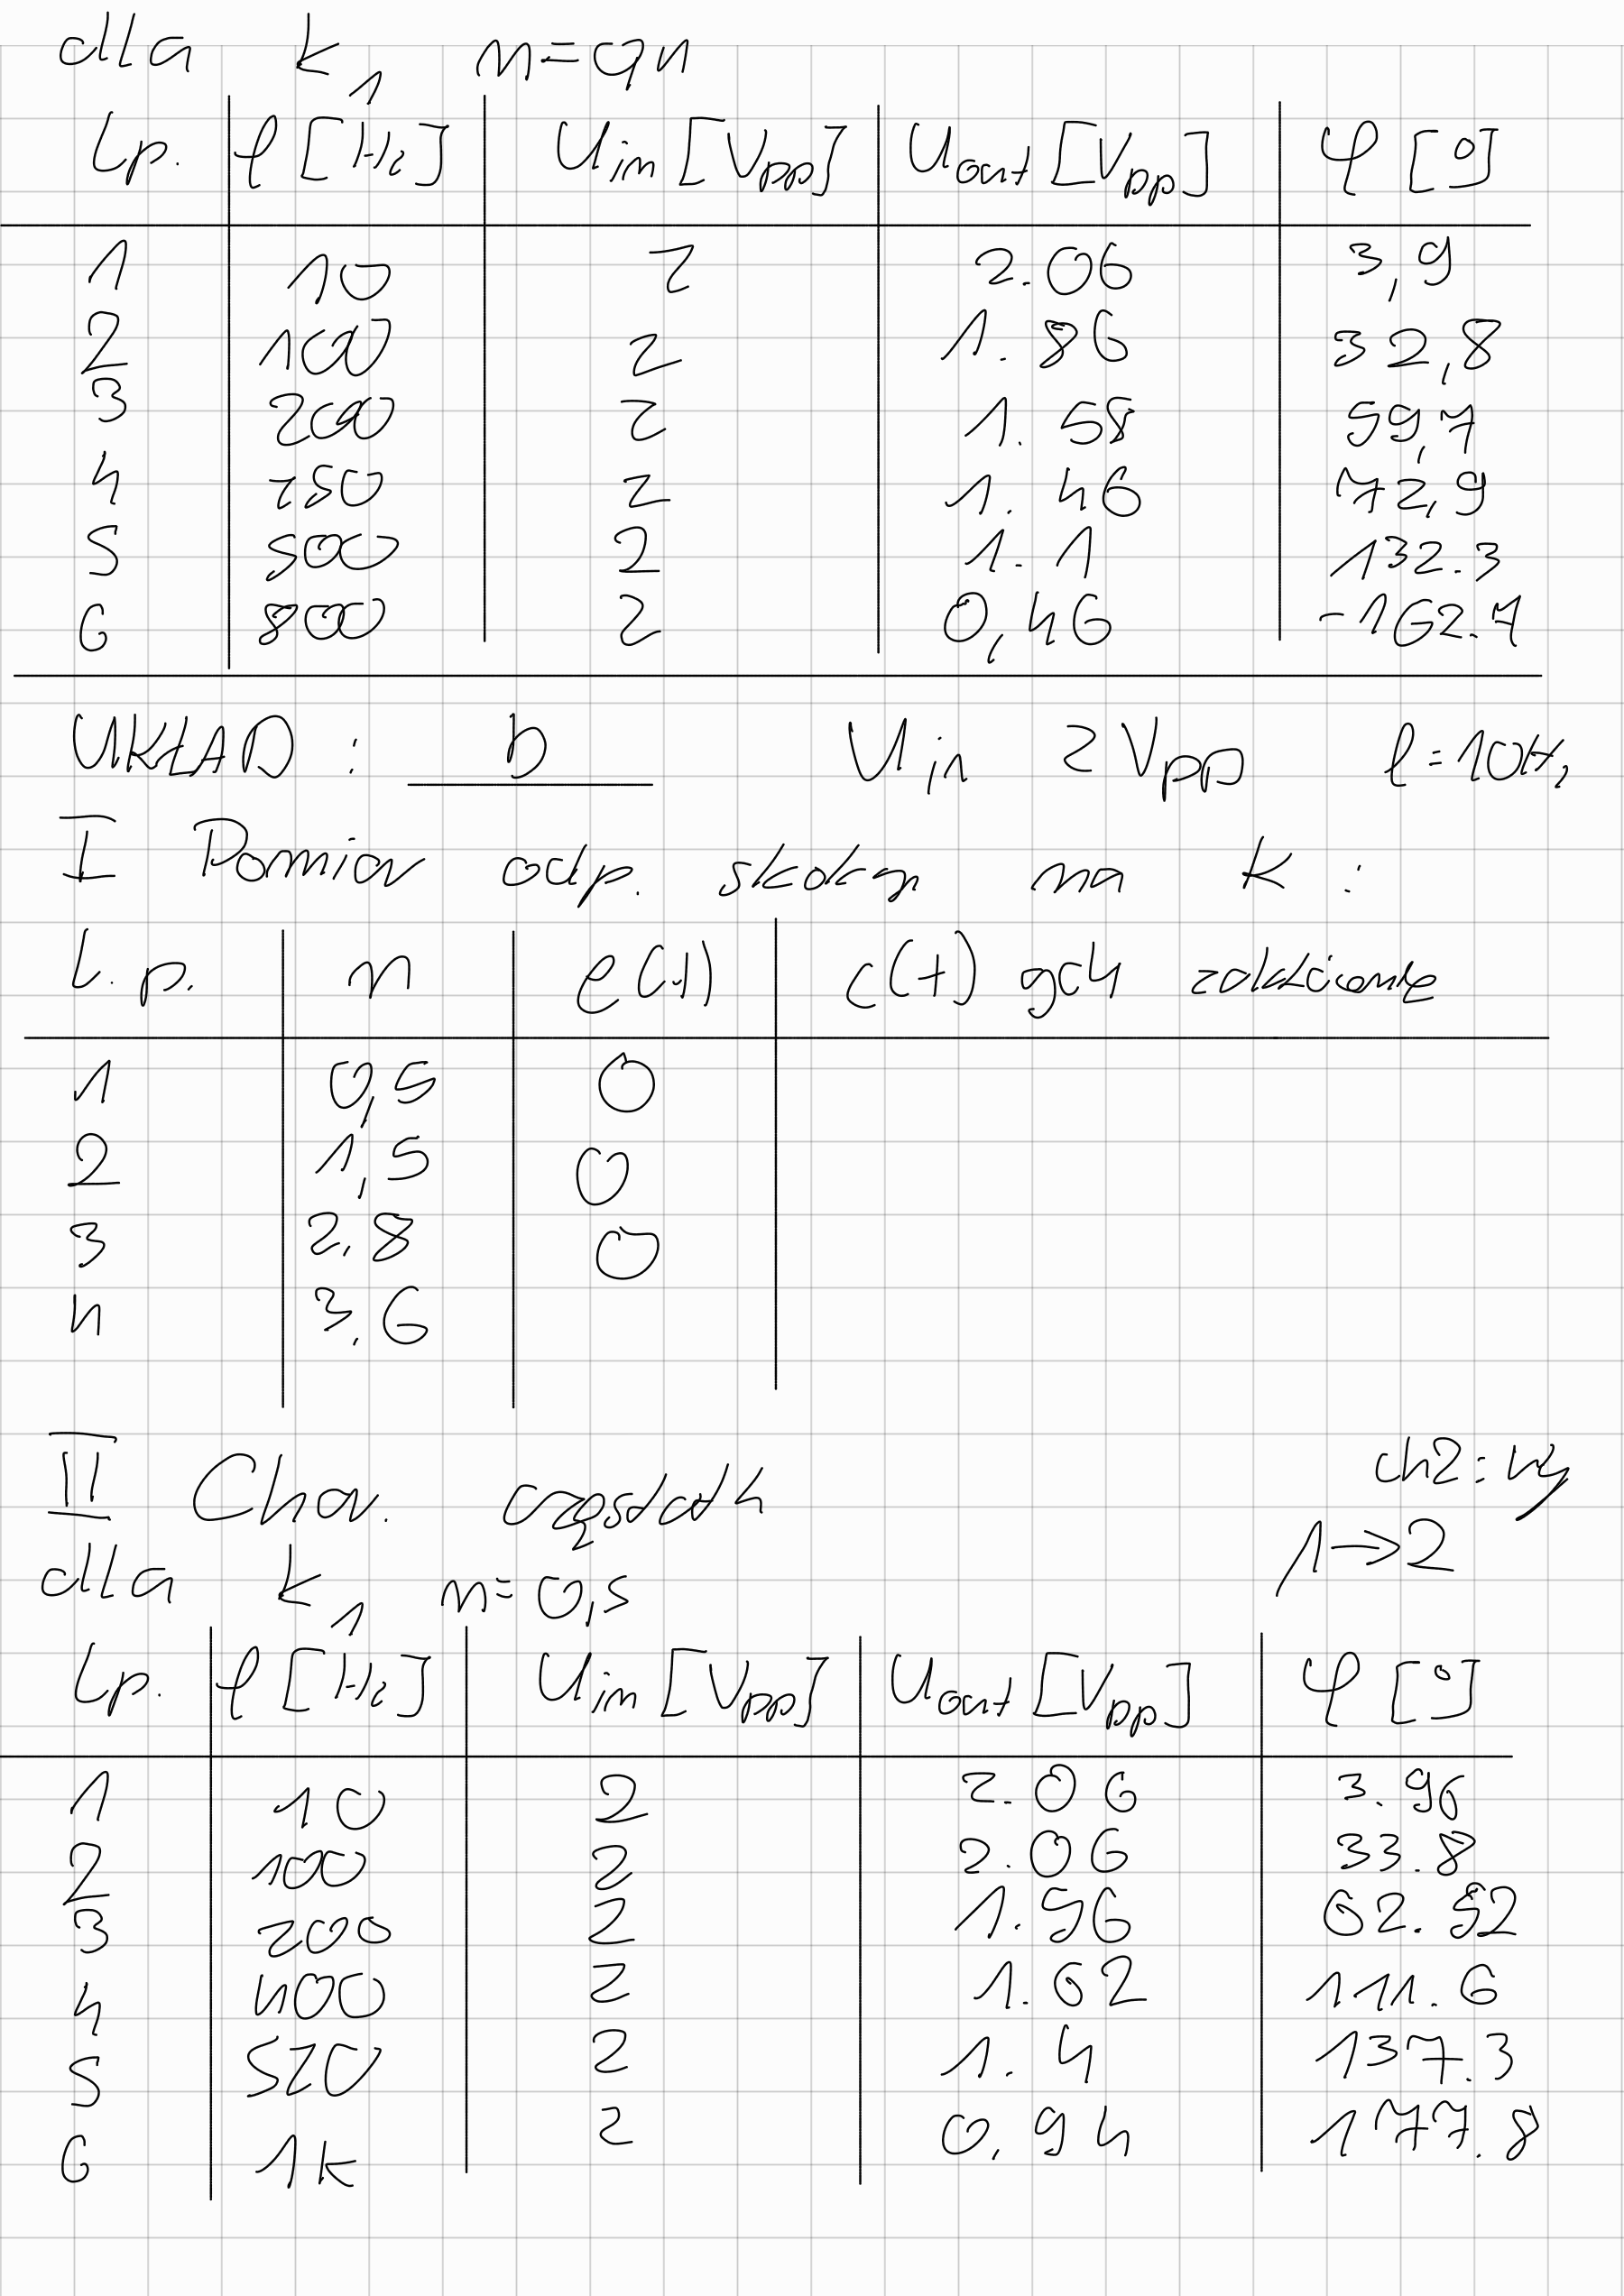
\includegraphics[width=\textwidth]{zdjecia/2.png}
			\caption{Zdjęcie pomiarów 2.}
			\label{fig:pomiar2}
		\end{subfigure}
		\caption{Zdjęcia wykonane podczas laboratorium.}
	\end{figure}
	
	\textbf {W ramach ćwiczenia dokonano identyfikacji następujących obiektów dynamicznych.}
	
	\subsection{Układ inercyjny pierwszego rzędu}
	Transmitancja obiektu ma postać:
	\begin{equation}
		G(s) = \frac{k_p}{1 + sT_p}
	\end{equation}
	gdzie: \(k_p\) – statyczne wzmocnienie układu, a \(T_p\) – stała czasowa obiektu.
	
	W celu identyfikacji obiektu inercyjnego pierwszego rzędu na jego wejście podano sygnał prostokątny o amplitudzie międzyszczytowej równej \(2\,\text{V}\). Odpowiedź skokowa systemu została zarejestrowana przy użyciu oscyloskopu cyfrowego, a dane pomiarowe zapisano w formacie CSV. Na podstawie zarejestrowanego przebiegu wyznaczono parametry układu za pomocą poniższych zależności.
	
	Wzmocnienie statyczne \(k_p\):
	\begin{equation}
		h(t)\big|_{t \to \infty} = k_p = \frac{y(\infty) - y(0)}{\Delta V_{in}}
	\end{equation}
	
	Stała czasowa \(T_p\):
	\begin{equation}
		h(t) = k_p(1-e^{-t/T_p})
	\end{equation}
	
	Podstawiając czas $t$ równy stałej czasowej $T_p$, otrzymujemy:
	\begin{equation}
		h(T_p) = k_p(1-e^{-T_p/T_p}) = k_p(1-e^{-1})
	\end{equation}
	
	Wartość $e^{-1}$ jest stałą i wynosi w przybliżeniu $0{,}368$, zatem:
	\begin{equation}
		h(T_p) \approx k_p(1-0{,}368) = 0{,}632 \cdot k_p
	\end{equation}
	
	Oznacza to, że po czasie równym stałej czasowej $T_p$ odpowiedź obiektu osiąga 63,2\% swojej wartości ustalonej.
	
	\textbf{Wyznaczone wartości parametrów układu są następujące:}
	\begin{itemize}
		\item $k_p = 0{,}871$
		\item $T_p = 0{,}78$ ms
	\end{itemize}
	
	\textbf{Parametry obliczone z charakterystyk częstotliwościowych:} \\
	\indent Wzmocnienie $k_p$ obliczono ze wzoru:
	
	\begin{equation}
		M(f)=\frac{A_{wy}}{A_{we}}
	\end{equation}
	
	Z pomiaru przy najniższej częstotliwości (10 Hz) mamy
	\begin{equation}
		k_p \approx M(10\ \text{Hz}) = \frac{1{,}71}{2{,}03} = 0{,}842.
	\end{equation}
	
	Wartość modułu przy częstotliwości granicznej spełnia
	\begin{equation}
		M(\omega_{3\text{dB}})=\frac{k_p}{\sqrt{2}} \approx \frac{0{,}842}{\sqrt{2}} = 0{,}595.
	\end{equation}
	
	Z tabeli widzimy, że częstotliwość wynosi:
	\[
	f_{3\text{dB}} \approx 210\ \text{Hz}.
	\]
	
	Stąd stała czasowa:
	\begin{equation}
		T_p = \frac{1}{\omega_{3\text{dB}}} = \frac{1}{2\pi f_{3\text{dB}}}
		\approx \frac{1}{2\pi\cdot 210} = 0{,}758\ \text{ms}.
	\end{equation}
	
	Dla częstotliwości granicznej $\omega_{3\text{dB}}$ zachodzi zależność:
	\begin{equation}
		\omega_{3\text{dB}} = \frac{1}{T_p} \approx 1319{,}3~\frac{\text{rad}}{\text{s}}
	\end{equation}
	
	\textbf{Parametry wyznaczone za pomocą skryptów MATLABowych:}
	\begin{itemize}
		\item $k_p = 0{,}8366$
		\item $T_p = 0{,}74$ ms
	\end{itemize}
	
	\textbf{Porównanie odpowiedzi skokowych modeli otrzymanych różnymi metodami:} \\
	Dane wejściowe: \\
	Vin = 2 [Vpp], f = 10 [Hz]
	
	\begin{figure}[H]
		\centering
		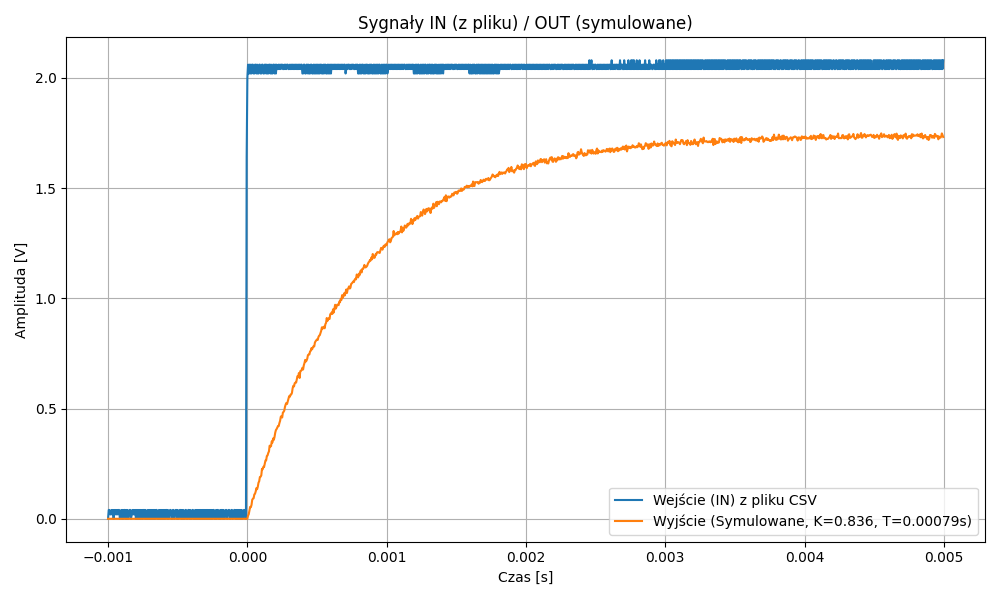
\includegraphics[width=1\linewidth]{zdjecia/OdpSkokowa1.png}
		\caption{Odpowiedzi skokowe układu inercyjnego pierwszego rzędu}
		\label{fig:OdpSkokowa1}
	\end{figure}
	
	\textbf{Porównanie charakterystyk Bodego otrzymanych różnymi metodami:}
	\begin{figure}[H]
		\centering
		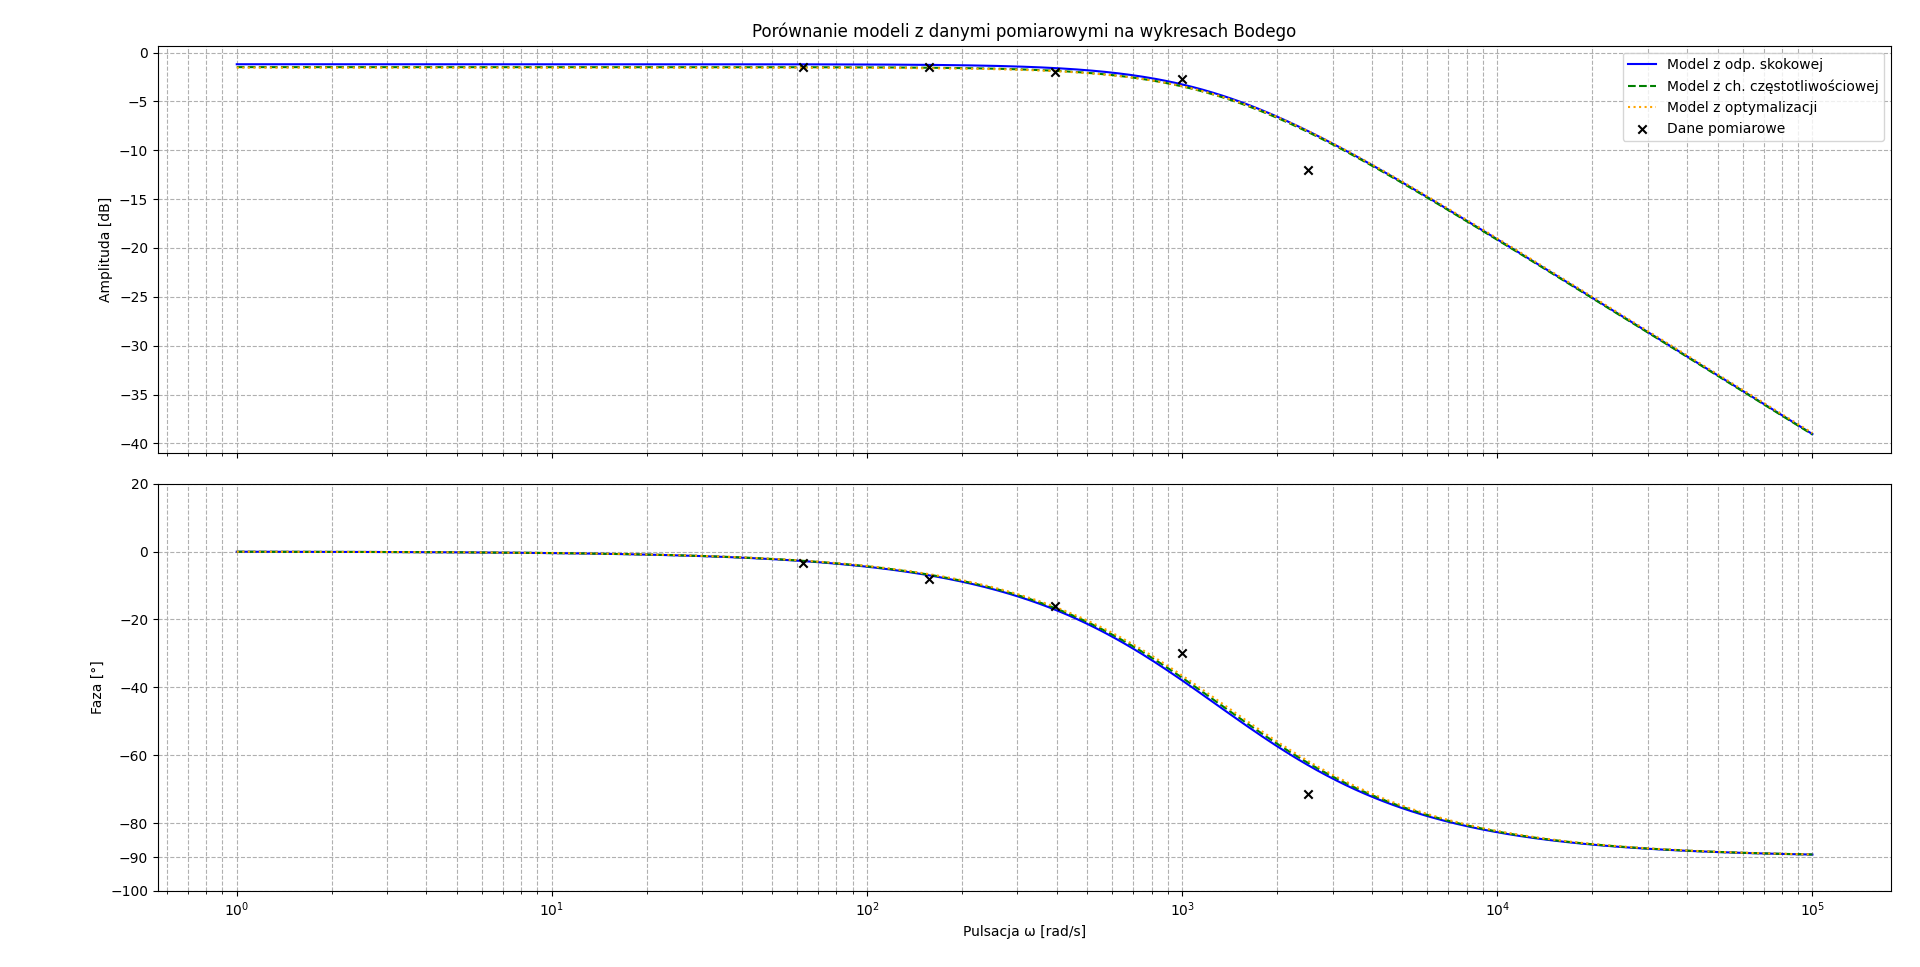
\includegraphics[width=1\linewidth]{zdjecia/Body1.png}
		\caption{Charakterystyki Bodego układu inercyjnego pierwszego rzędu}
		\label{fig:Body1}
	\end{figure}
	
	Porównanie parametrów uzyskanych za pomocą trzech różnych metod identyfikacji wykazało bardzo dużą zgodność, która jest potwierdzona wizualnie na wykresach (Rysunek 2 i Rysunek 3). Świadczy to o wiarygodności wykonanych pomiarów oraz poprawności przyjętego modelu matematycznego. Zarejestrowana odpowiedź skokowa, przedstawiona na Rysunku 2, nie wykazuje przeregulowania, co stanowi typową cechę tego typu systemów. Właściwości obiektu jako filtru dolnoprzepustowego przejawiają się w tłumieniu składowych o wysokich częstotliwościach oraz w przesunięciu fazowym, które dla dużych częstotliwości dąży do -90° (Rysunek 3).
	
	\subsection{Układ inercyjny pierwszego rzędu z opóźnieniem transportowym}
	Transmitancja obiektu ma postać:
	\begin{equation}
		G(s) = \frac{k_p}{1 + sT_p} e^{-sT_0}
	\end{equation}
	gdzie: \(k_p\) – statyczne wzmocnienie układu, \(T_p\) – stała czasowa obiektu, a \(T_0\) - opóźnienie transportowe.
	
	Parametry $k_p$ i $T_p$ przyjęto takie same jak dla układu inercyjnego pierwszego rzędu, ponieważ wprowadzenie opóźnienia transportowego $T_0$ nie wpływa na wzmocnienie ani stałą czasową, a jedynie powoduje dodatkowe przesunięcie fazowe.
	
	\textbf{Obliczenie opóźnienia transportowego $T_0$ na podstawie odpowiedzi skokowej:}
	\begin{figure}[H]
		\centering
		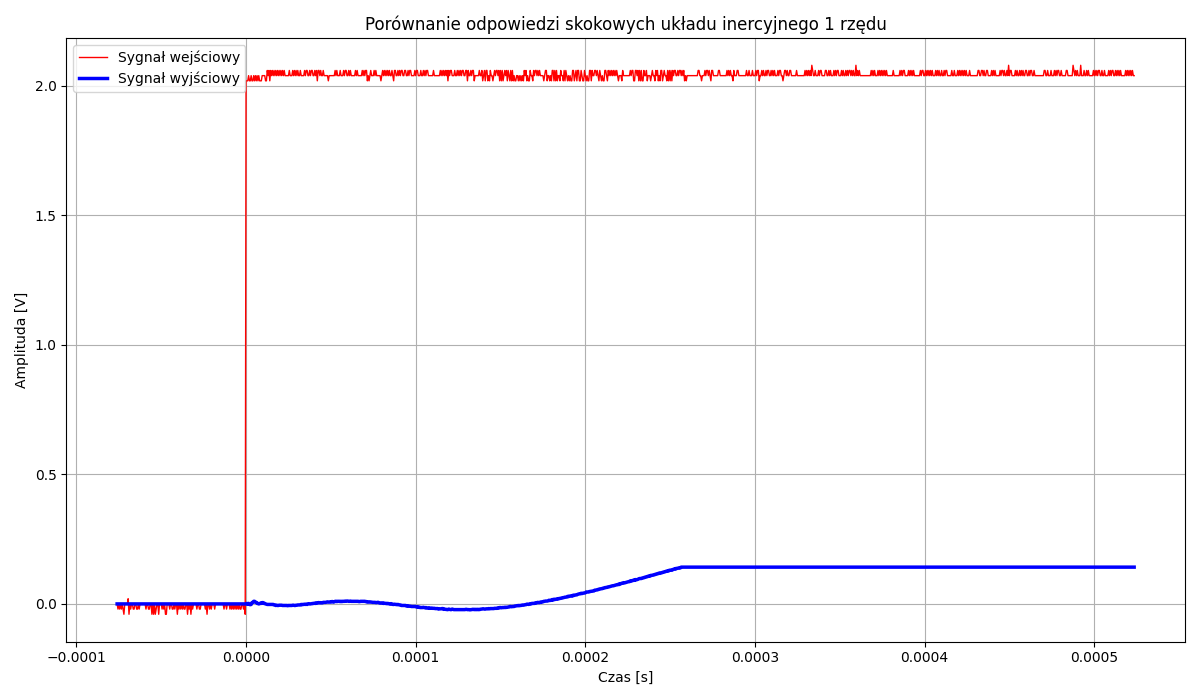
\includegraphics[width=1\linewidth]{zdjecia/odp_skok_z_opz.png}
		\caption{Odpowiedź skokowa układu pierwszego rzędu z opóźnieniem transportowym}
		\label{fig:odp_skok_z_opz}
	\end{figure}
	
	\textbf{Wyznaczone wartości parametrów układu są następujące:}
	\begin{itemize}
		\item $k_p = 0{,}871$
		\item $T_p = 0{,}78$ ms
		\item $T_0 = 0{,}175$ ms
	\end{itemize}
	
	\textbf{Obliczenie opóźnienia transportowego $T_0$ na podstawie charakterystyki częstotliwościowej:}
	\begin{equation}
		T_0 = -T_p \cdot \left( \phi(\omega_{3\text{dB}}) + \frac{\pi}{4} \right)
	\end{equation}
	
	Do obliczeń przyjęto $T_p = 0{,}758~\text{ms}$ oraz przesunięcie fazowe $\phi = -71{,}88^{\circ}$ (odczytane dla częstotliwości $f = 210~\text{Hz}$, bliskiej $f_{3\text{dB}}$).
	
	Konwersja fazy na radiany:
	\[
	\phi = -71{,}88^{\circ} = -1{,}2545~\text{rad}
	\]
	
	Podstawienie wartości do wzoru:
	\begin{align*}
		T_0 &= -0{,}000758~\text{s} \cdot \left( -1{,}2545 + \frac{\pi}{4} \right) \\
		T_0 &= -0{,}000758~\text{s} \cdot \left( -1{,}2545 + 0{,}7854 \right) \\
		T_0 &= -0{,}000758~\text{s} \cdot (-0{,}4691) \\
		T_0 &\approx 0{,}000356~\text{s}
	\end{align*}
	
	Ostatecznie wyznaczone opóźnienie transportowe wynosi:
	\[
	\boxed{T_0 \approx 0{,}356~\text{ms}}
	\]
	
	\textbf{Porównanie charakterystyk Bodego otrzymanych różnymi metodami:}
	\begin{figure}[H]
		\centering
		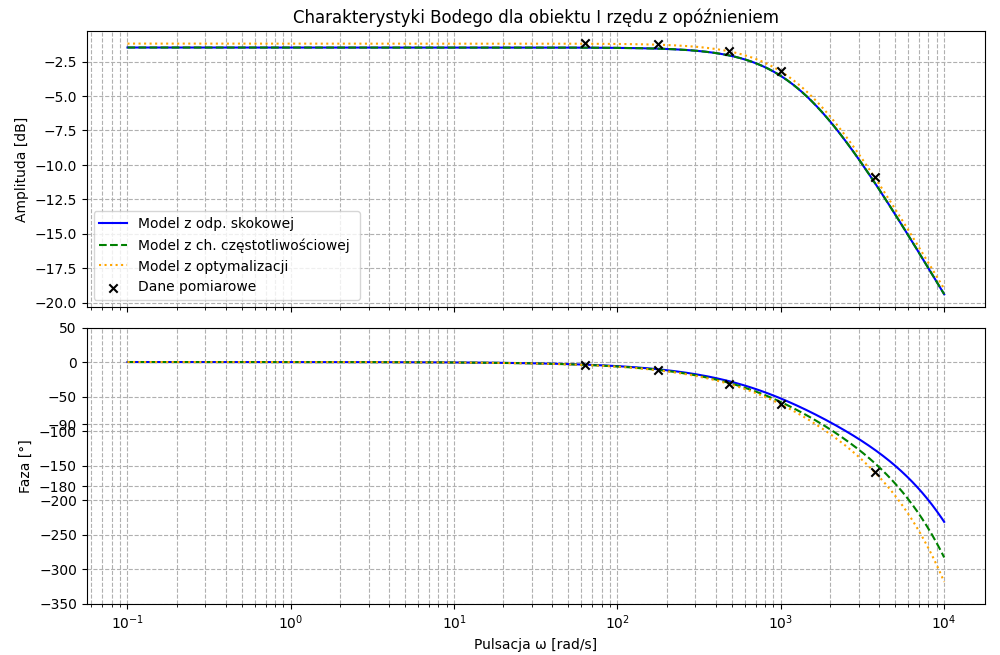
\includegraphics[width=1\linewidth]{zdjecia/1rzad_z_opz.png}
		\caption{Charakterystyki Bodego układu inercyjnego pierwszego rzędu z opóźnieniem transportowym.}
		\label{fig:Body1_z_opz}
	\end{figure}
	
	Charakterystyka amplitudowa potwierdza, że obiekt zachowuje się jak filtr dolnoprzepustowy, tłumiąc składowe o wysokich częstotliwościach. W odróżnieniu od układu inercyjnego bez opóźnienia, charakterystyka fazowa wykazuje znacznie większe przesunięcie ujemne, które systematycznie maleje wraz ze wzrostem częstotliwości. Jest to charakterystyczna cecha systemów z opóźnieniem transportowym, gdzie opóźnienie wprowadza dodatkowe, przesunięcie fazowe.
	
	\subsection{Układ całkujący}
	Transmitancja obiektu jest postaci:
	\begin{equation}
		G(s) = \frac{1}{sT_i}
	\end{equation}
	gdzie: \(T_i\) – stała całkowania.
	
	\textbf{Porównanie sygnałów wyjściowych pobudzonych różnymi napięciami:}
	\begin{figure}[H]
		\centering
		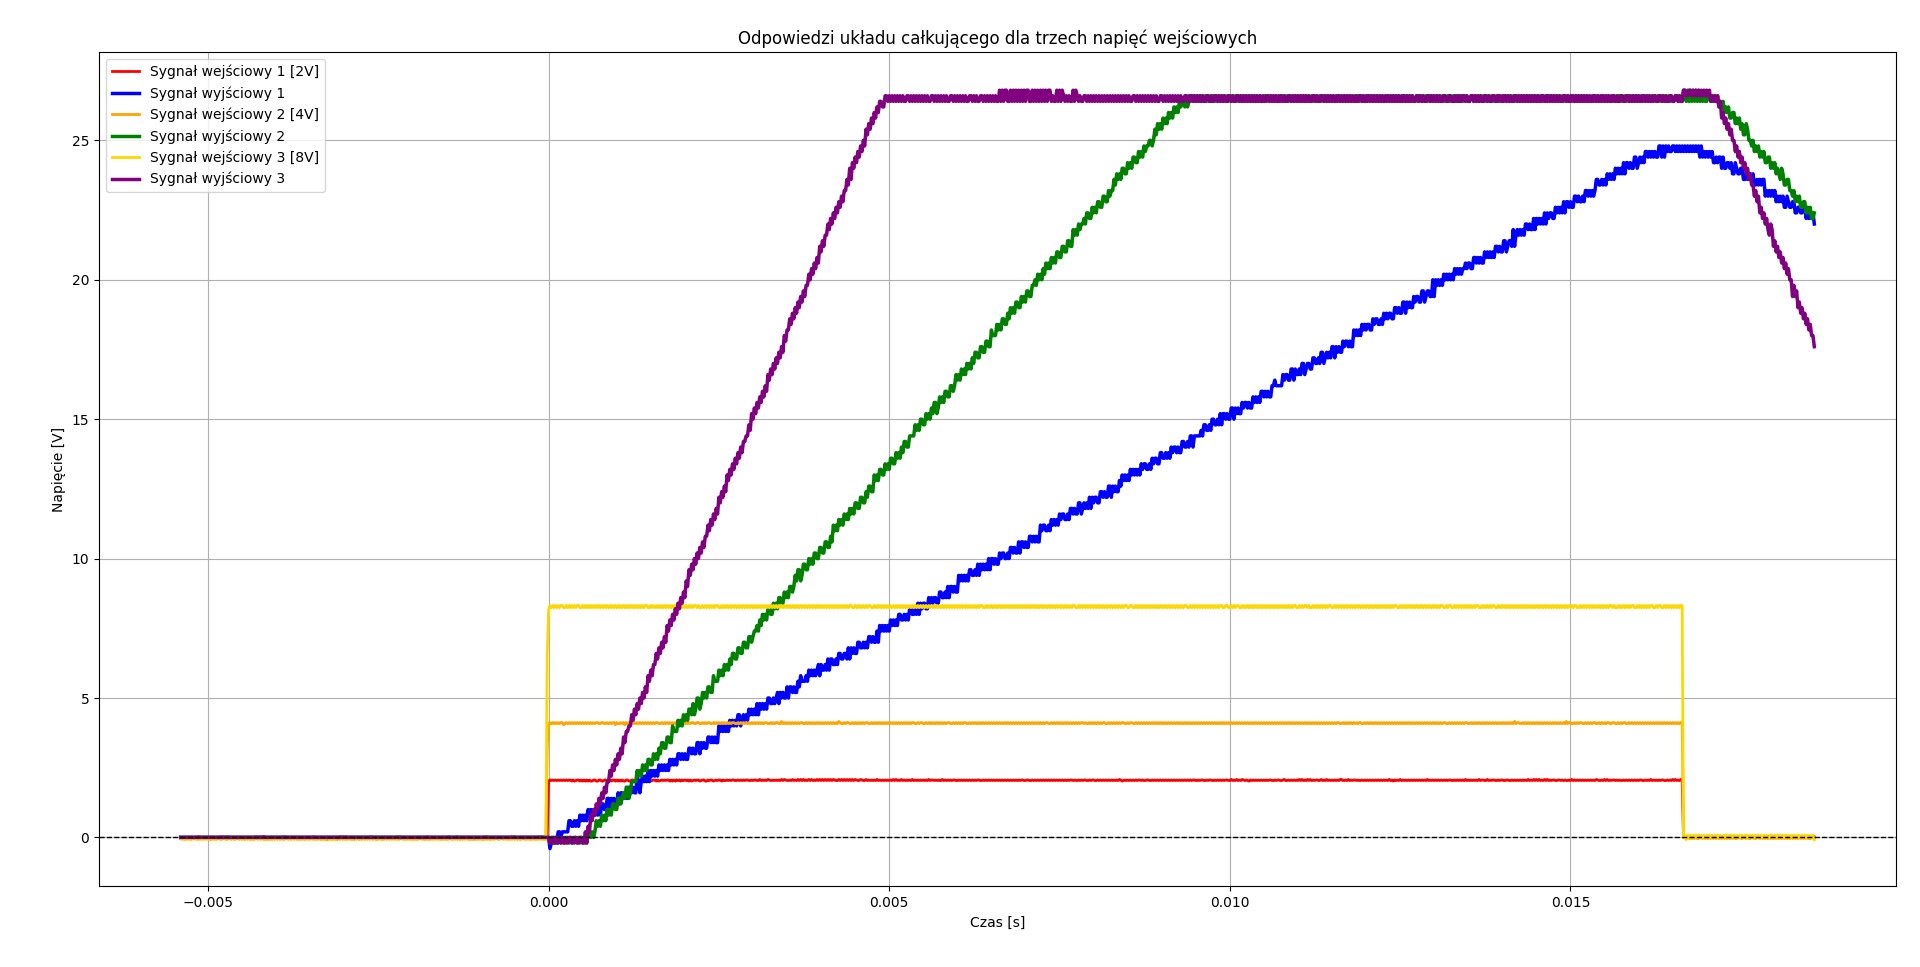
\includegraphics[width=0.8\textwidth]{zdjecia/UkladCalk.png}
		\caption{Odpowiedź układu całkującego na różne napięcia wejściowe.}
		\label{fig:uklad_calk}
	\end{figure}
	
	\textbf{Obliczenie stałej całkowania $T_i$ na podstawie danych pomiarowych:}
	\[
	T_i = \frac{\Delta U_{we} \cdot \Delta x}{\Delta y}
	\]
	\begin{itemize}
		\item $\Delta U_{we}$ - Zmiana amplitudy sygnału wejściowego [V]
		\item $\Delta x$ - Różnica czasu [s]
		\item $\Delta y$ - Różnica napięcia [V]
		\item $T_i$ - Stała całkowania [s]
	\end{itemize}
	
	\begin{table}[h!]
		\centering
		\begin{tabular}{|c|c|c|c|}
			\hline
			$\Delta U_{we}$ [V] & $\Delta x$ [s] & $\Delta y$ [V] & $T_i$ [ms] \\
			\hline
			2 & 0,0092 & 14,5 & 1,27 \\
			4 & 0,0069 & 21,6 & 1,28 \\
			8 & 0,0036 & 21,6 & 1,33 \\
			\hline
		\end{tabular}
	\end{table}
	
	\[
	T_{i\,\text{średnie}} = \frac{1,27 + 1,28 + 1,33}{3} = 1,29\ \text{ms}
	\]
	
	Dla różnych wartości napięcia wejściowego obserwowano liniowy wzrost napięcia wyjściowego w funkcji czasu, co wskazuje na proporcjonalność prędkości narastania sygnału do amplitudy wymuszenia. Wyznaczone wartości stałej całkowania Ti dla trzech pomiarów są do siebie bardzo zbliżone ($T_isrednie = 1,29 ms$), co potwierdza poprawność pomiarów i stabilność układu.
	
	
	\subsection{Układ drugiego rzędu}
	Transmitancja obiektu jest postaci:
	\begin{equation}
		G(s) = \frac{1}{1 + sa_1 + s^2a_2}
		= \frac{1}{1+s 2\zeta \tau + s^2 \tau^2}
		= \frac{w_n^2}{w_n^2 + s 2 \zeta w_n + s^2}
	\end{equation}
	gdzie: \(\zeta\) – współczynnik tłumienia, \(w_n = \frac{1}{\tau}\) – pulsacja naturalna (drgań nietłumionych).
	
		\textbf {Obliczone parmatrey układu 2 rzędu na podstawie odpowiedzi skokowej}
	
	DO ZMIANY JAK USTALIMY WARTOŚCI ODPOWIEDNIE
	
	\begin{itemize}
		\item $\kappa = 0.2544 $
		\item $T_\kappa = 1,370 ms$
		\item $\xi = 0,3995$
		\item $\tau = 0,4 ms$
	\end{itemize}
	
	\textbf{Wartości oparte o charakterystyke czestotliwościową}
	
	\textbf{Wartość wyznaczone na podstawie optymalizacji}
	\begin{itemize}
		\item $\xi = 0,129$
		\item $\omega = 5406$
	\end{itemize}
	
	\subsection{Układ nieminimalnofazowy}
	Transmitancja obiektu jest postaci:
	\begin{equation}
		G(s) = \frac{1-sT_x}{1+sT_y}
	\end{equation}
	gdzie: \(T_x\) – stała czasowa zera, \(T_y\) – stała czasowa bieguna.
	

	
	\begin{itemize}
		\item 
	\end{itemize}
	
	\section{Wnioski}
	
\end{document}
